% start the document

% specify the document layout and font size
\documentclass[preprint,12pt]{elsarticle}
% \documentclass[final,twocolumn,12pt]{elsarticle}
\usepackage[margin=1.5cm,includefoot]{geometry}
\usepackage{setspace}

% uploading packages
\usepackage{graphicx}
\usepackage{amssymb}
\usepackage{textcomp} % https://latex.org/forum/viewtopic.php?f=4&t=3364#p13124, https://tex.stackexchange.com/questions/165115
\usepackage{gensymb}
\usepackage{lineno}
\usepackage{mathtools}
\usepackage[title]{appendix}
\usepackage[separate-uncertainty=true]{siunitx}
\usepackage{xr-hyper} %needs to  be before hyperref
\usepackage[colorlinks]{hyperref}
\usepackage[nameinlink,capitalise]{cleveref} %needs to appear after hyperref, https://tex.stackexchange.com/questions/396728/my-equations-referencing-not-working
\Crefname{figure}{Figure}{Figures} %needs to appear after hyperref and cleveref
\crefname{appsec}{Appendix}{Appendices}
\newcommand\crefrangeconjunction{--} % modify the reference style
\usepackage{mathrsfs}
\usepackage{url}
\usepackage{enumitem}
\usepackage{tabulary}
\usepackage{caption}
\usepackage{subcaption}
\usepackage{multirow}
\usepackage{makecell} % https://tex.stackexchange.com/questions/2441/how-to-add-a-forced-line-break-inside-a-table-cell
\newcommand{\NA}{---} % holds an m-dash
\graphicspath{{figures/}} %Setting the graphicspath
% ---------to deal with the double quotes----------- 
\usepackage [english]{babel}
\usepackage [autostyle, english = american]{csquotes}
\MakeOuterQuote{"}
%alternatively can use `` '' format for double quotes
\usepackage{booktabs}
\setlength{\abovetopsep}{1ex}
\usepackage[shortcuts,abbreviations]{glossaries-extra}
\newcommand*{\TCac}[1]{\ecapitalisewords{\glsentrylong{#1}}}

% remove the "Preprint submitted to Elsevier" footer on the first page
\makeatletter
\def\ps@pprintTitle{%
   \let\@oddhead\@empty
   \let\@evenhead\@empty
   \def\@oddfoot{\reset@font\hfil\thepage\hfil}
   \let\@evenfoot\@oddfoot
}
\makeatother

% Add "S" to figure captions
\renewcommand{\thefigure}{S\arabic{figure}}
\renewcommand{\thesection}{S\arabic{section}}

% Cross referencing with the xr package in Overleaf (https://www.overleaf.com/learn/how-to/Cross_referencing_with_the_xr_package_in_Overleaf)
\makeatletter
\newcommand*{\addFileDependency}[1]{% argument=file name and extension
  \typeout{(#1)}
  \@addtofilelist{#1}
  \IfFileExists{#1}{}{\typeout{No file #1.}}
}
\makeatother
\newcommand*{\myexternaldocument}[1]{%
    \externaldocument{#1}%
    \addFileDependency{#1.tex}%
    \addFileDependency{#1.aux}%
}

\usepackage{nameref,zref-xr}
\zxrsetup{toltxlabel}
\zexternaldocument*{main}

% % figure info, etc. that can dynamically change (color of points, etc.)
% \newcommand{\startpt}{red points}
% \newcommand{\singlept}{magenta points}
% \newcommand{\sympt}{dark blue points}
% \newcommand{\singlesympt}{dark blue point}
% \newcommand{\refpt}{white circle}
% \newcommand{\vbordercolor}{black}
% \newcommand{\vcellcolor}{light blue}
\newcommand{\inpt}{input}
\newcommand{\outpt}{prediction}
% \newcommand{\inptvar}{nmeshpts}
% \newcommand{\distfn}{GBdist4}

\newcommand{\vfzorepo}{\gls{vfzo} repository}

% %RMSE values
% \newcommand{\baryrmse}{0.0242}
% \newcommand{\gprrmse}{0.0220}
% \newcommand{\idwrmse}{0.0345}
% \newcommand{\nnrmse}{0.0448}
% \newcommand{\avgrmse}{0.1302}

% %MAE values
% \newcommand{\barymae}{0.0145}
% \newcommand{\gprmae}{0.0145}
% \newcommand{\idwmae}{0.0223}
% \newcommand{\nnmae}{0.0307}
% \newcommand{\avgmae}{0.0965}

% \newcommand{\nnomega}{2.8568 \pm 0.70121}

% \newcommand{\symtime}{76}

\newcommand{\thr}{\SI{1.2}{\joule\per\square\meter}}
\newcommand{\sigthr}{\SI{1.1}{\joule\per\square\meter}}

\glssetcategoryattribute{abbreviation}{indexonlyfirst}{true}
\glssetcategoryattribute{abbreviation}{nohyper}{true}
\makeglossaries

\newabbreviation{5dof}{5DOF}{five degree-of-freedom}
\newabbreviation{ebsd}{EBSD}{electron backscatter diffraction}
\newabbreviation[longplural={grain boundaries}]{gb}{GB}{grain boundary}
\newabbreviation{fcc}{FCC}{face-centered cubic}
\newabbreviation{mfc}{MFC}{mass flow controller}
\newabbreviation{sem}{SEM}{scanning electron microscope}
\newabbreviation{fea}{FEA}{finite element analysis}
\newabbreviation{bcs}{BCs}{boundary conditions}
\newabbreviation[longplural={triple junctions}]{tj}{TJ}{triple junction}
\newabbreviation{gpr}{GPR}{Gaussian process regression}
\newabbreviation{ann}{ANN}{artificial neural network}
\newabbreviation{nn}{NN}{nearest neighbor}
\newabbreviation{rmse}{RMSE}{root mean square error}
\newabbreviation{mae}{MAE}{mean absolute error}
\newabbreviation{brk}{BRK}{Bulatov Reed Kumar}
\newabbreviation{gbed}{GBED}{grain boundary energy distribution}
\newabbreviation{gbcd}{GBCD}{grain boundary character distribution}
\newabbreviation{mfz}{MFZ}{misorientation fundamental zone}
\newabbreviation{bp}{BP}{boundary plane}
\newabbreviation{knn}{kNN}{k-nearest neighbor}
\newabbreviation{gbe}{GBE}{grain boundary energy}
\newabbreviation{gbo}{GBO}{grain boundary octonion}
\newabbreviation{oslerp}{oSLERP}{octonion Spherical Linear Interpolation}
\newabbreviation{loocv}{LOOCV}{leave-one-out cross validation}
\newabbreviation{kfcv}{kFCV}{k-fold cross validation}
\newabbreviation{seo}{SEO}{symmetrically equivalent octonion}
\newabbreviation{fex}{FEX}{file exchange}
\newabbreviation{idw}{IDW}{inverse-distance weighting}
\newabbreviation{fic}{FIC}{fully independent conditional}
\newabbreviation{svd}{SVD}{singular value decomposition}
\newabbreviation{gbc}{GBC}{grain boundary character}
\newabbreviation{fz}{FZ}{fundamental zone}
% \newabbreviation{pfz}{pFZ}{pseudo fundamental zone} % pfz replaced by vfz
% \newabbreviation{cmo}{CMO}{closed-mesh octonion} % cmo replaced by vfzo
\newabbreviation{vfz}{VFZ}{Voronoi Fundamental Zone}
\newabbreviation{vfzo}{VFZO}{Voronoi Fundamental Zone octonion}
\newabbreviation{lobpcg}{LOBPCG}{locally optimal block preconditioned conjugate gradient}
\newabbreviation{lkr}{LKR}{Laplacian kernel regression}
% example abbreviations
% \newabbreviation{seo}{SEO}{symmetrically equivalent octonions}
%\newabbreviation[longplural={grain boundaries}]{gb}{GB}{grain boundary}

%example usage: \gls{gpr}
%example usage: \Gls{gpr} (capitalize first letter, only meaningful for first usage)
% \glspl{seo} --> symmetrically equivalent octonions OR SEOs
%^^^^^^^^^^^^^^^^^^^^^^^^^^^^^^^^^^^^^^^^^^^^^^^^^^^

\biboptions{sort&compress}
\interfootnotelinepenalty=10000
\patchcmd{\emailauthor}{(#2)}{(O.K. Johnson).}{}{}
% Double Spacing
% \doublespacing
\begin{document}

\begin{frontmatter}

%\title{Grain Boundary Octonion Meshing and Interpolation}
\title{Five Degree-of-Freedom Property Interpolation of Arbitrary Grain Boundaries via \glsentrytitlecase{vfzo}{long} Framework: Supplementary Information}

\author[myu]{Sterling G. Baird}
\author[myu]{Eric R. Homer}
\author[myu]{David T. Fullwood}
\author[myu]{Oliver K. Johnson\corref{cor1}}
\ead{ojohnson@byu.edu}

\address[myu]{Department of Mechanical Engineering, Brigham Young University, Provo, UT 84602, USA}

\cortext[cor1]{Corresponding author.}

\date{October 2020}
\end{frontmatter}

\section{Euclidean and Arc Length Distances}
\label{sec:supp:dist-parity}
The close correlation between Euclidean and arc length distances in the \gls{vfzo} sense is shown in \cref{fig:dist-parity}.


\begin{figure}[h!]
\centering
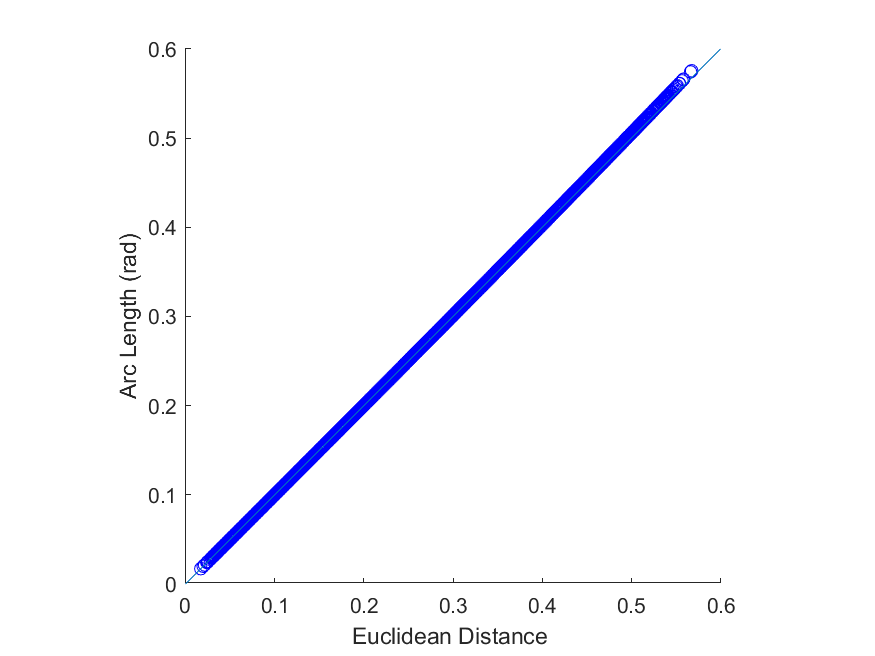
\includegraphics[scale=1]{dist-parity.png}
\caption{Parity plot of 8D Cartesian hyperspherical arc length vs. 8D Cartesian Euclidean distance for pairwise distances in a ($m\bar{3}m$) symmetrized set of \num{10000} randomly sampled \glspl{vfzo}. The max arc length is approximately \SI{0.58}{\radian}, indicating a max octonion distance of approximately \SI{1.16}{\radian} or \SI{66.5}{\degree} between any two points in the \gls{vfz}. The close correlation between arc length and Euclidean distance supports the validity of using Euclidean distance instead of arc length in the interpolation methods. This is \textit{separate} from the correlation between \gls{vfzo} Euclidean or arc length distances with the traditional octonion distance \cite{chesserLearningGrainBoundary2020}.}
\label{fig:dist-parity}
\end{figure}

\section{Barycentric Interpolation}
\label{sec:supp:bary}

\subsection{High-Aspect Ratios}
\label{sec:supp:bary:artifact}
An artifact of the barycentric interpolation method which occurs due to the presence of high-aspect ratio facets is shown in \cref{fig:high-aspect-non-int}. As the dimensionality increases for a constant number of points and from our numerical tests, the rate of missed facet intersections increases. This artifact, and our method for addressing it, are discussed in \cref{sec:app:bary:int}.

\begin{figure*}
    \centering
    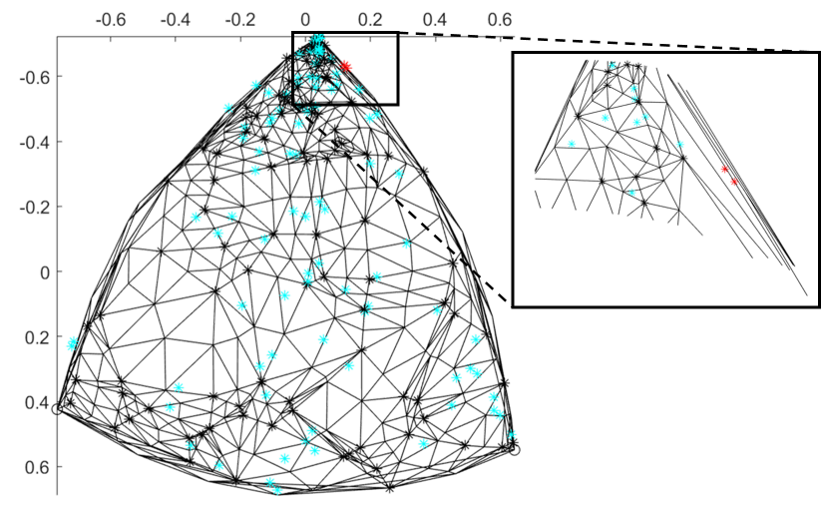
\includegraphics[scale=1]{figures/high-aspect-non-int.png}
    \caption{Illustration of two \outpt{} points (red) for which no intersecting facet is found due to being positioned within a high-aspect ratio facet. The inset shows that facets connected to the \gls{nn} do not contain the \outpt{} point. Many \glspl{nn} would need to be considered before an intersection is found. Additionally, it is expected that if found, the interpolation will suffer from higher error due to use of facet vertices far from the interpolation point. Proper intersections of \outpt{} points with the mesh are shown in blue.}
    \label{fig:high-aspect-non-int}
\end{figure*}

% \subsection{Use of Alternative Distance Metrics}


\section{Kim Interpolation}
\label{sec:supp:kim-interp}

A \gls{gpr} mixing model is developed to accommodate the non-uniformly distributed, noisy Fe simulation data \cite{kimPhasefieldModeling3D2014} and better predict low \gls{gbe}. Details of the method (\cref{sec:supp:kim-interp:method}) and an analysis of the input data quality (\cref{sec:supp:kim-interp:quality}) are given. The code implementation is given in \texttt{gprmix.m} and \texttt{gprmix\_test.m} of the \vfzorepo{} \cite{bairdFiveDegreeofFreedom5DOF2020}.

\subsection{Details of \glsentrytitlecase{gpr}{long} Mixture}
\label{sec:supp:kim-interp:method}
As shown in \cref{fig:kim-interp-teach}d, prediction using the standard approach of the main document overestimates low \glspl{gbe} (termed the $\epsilon_1$ model). By training the data on only \glspl{gb} with a \gls{gbe} less than \thr{} (termed the $\epsilon_2$ model) and by using an exponential (\texttt{KernelFunction='exponential'}) rather than a squared exponential kernel, prediction of low \glspl{gbe} improves, but naturally underestimation occurs for higher \glspl{gbe} (\cref{fig:kim-interp-teach}c).

\begin{figure}
    \centering
    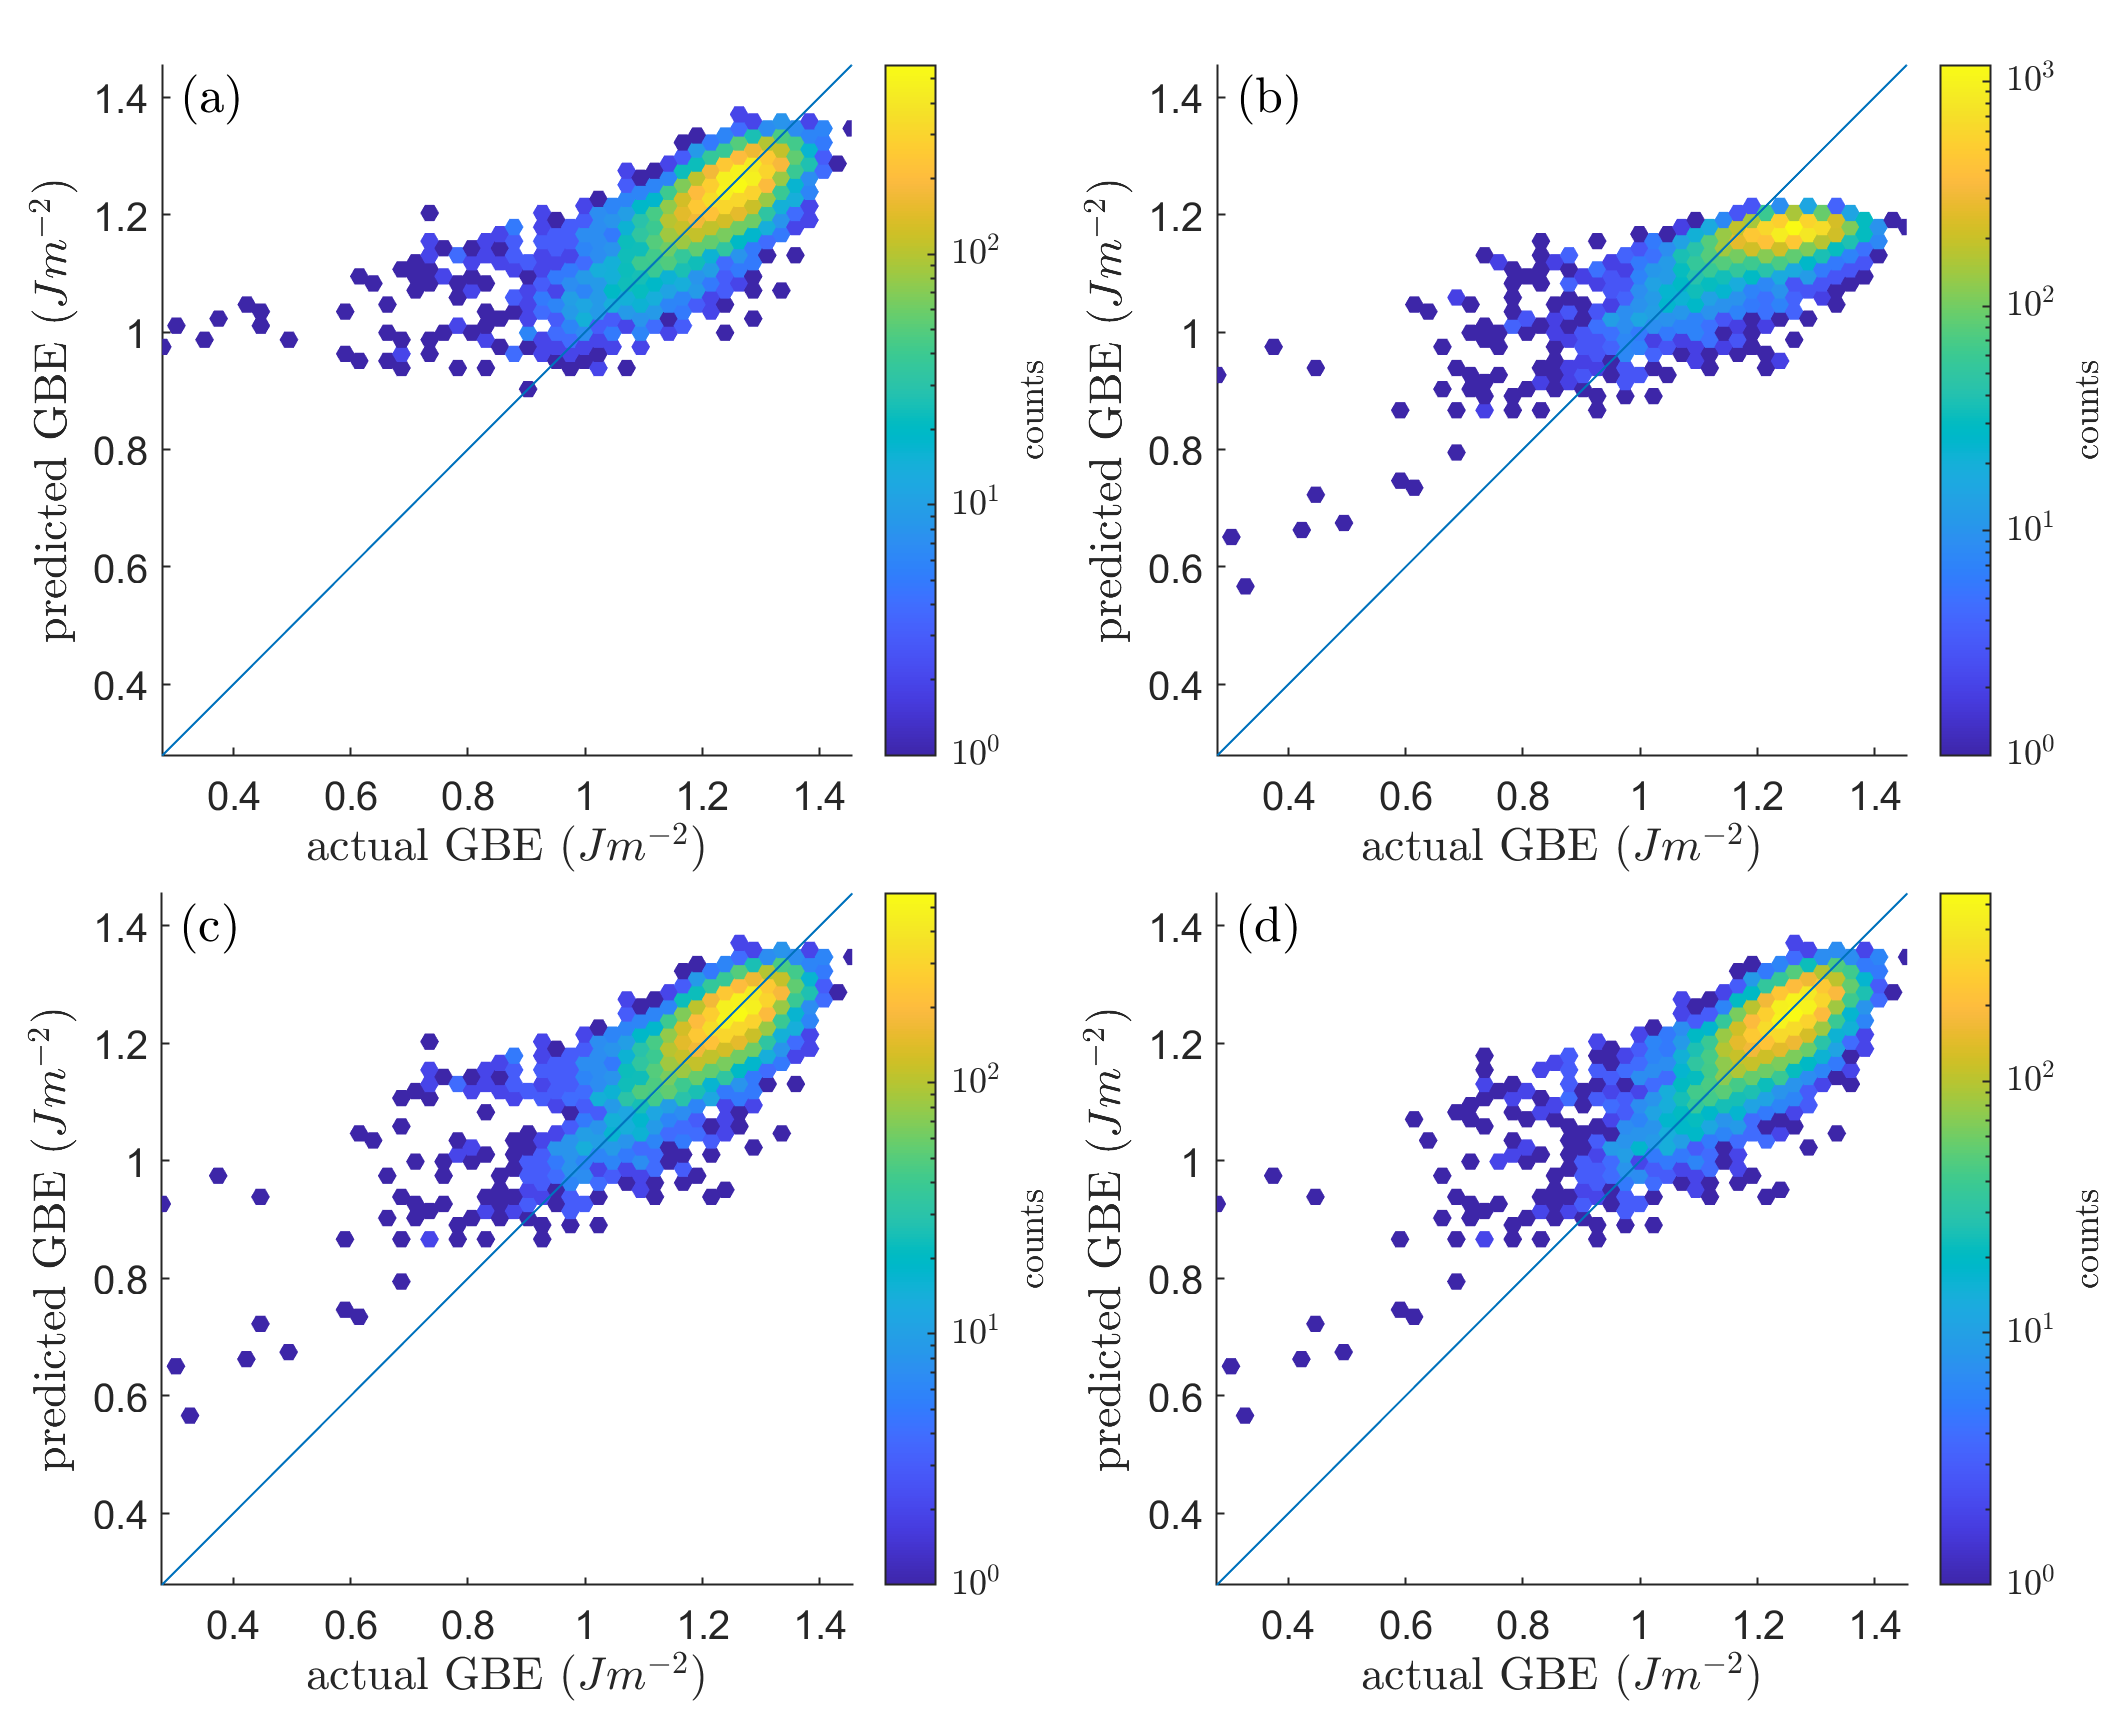
\includegraphics{kim-interp-teach.png}
    \caption{Teaching figure to demonstrate the \gls{gpr} mixing model. Hexagonally binned parity plot of the standard \gls{gpr} model (a). All prediction \glspl{gb} based on the model using only training \glspl{gb} with a \gls{gbe} less than \thr{} (b). Selected points from each of the two models to be mixed (c), and hexagonally binned parity plots of the \gls{gpr} mixing model (d). Points in (c) are produced by splitting the prediction data into less than and greater than \thr{}. A sigmoid mixing function (\cref{fig:gprmix-sigmoid}) is then applied where the predicted \glspl{gbe} shown in (c) determines the mixing fraction (f) to produce a weighted average of models (b) and (a). A large Fe simulation database \cite{kimPhasefieldModeling3D2014} using \num{46883} training datapoints and \num{11721} validation datapoints in an 80\%/20\% split is used. The \gls{gpr} mixture model decreases error for low \gls{gbe} (d) and changes overall \gls{rmse} and \gls{mae} from \SI{0.057932}{\J\per\square\meter} and \SI{0.039857}{\J\per\square\meter} in the original model (a) to \SI{0.057502}{\J\per\square\meter} and \SI{0.041272}{\J\per\square\meter}, respectively.}
    \label{fig:kim-interp-teach}
\end{figure}

A combined, disjoint model (\cref{fig:kim-interp-teach}b) is taken ($\epsilon_3$) by replacing $\epsilon_1$ \gls{gbe} predictions for \glspl{gb} with \gls{gbe} less than \thr{} with the corresponding $\epsilon_2$ predictions. Finally, a weighted average (\cref{eq:gprmix}) is taken according to:

\begin{equation}
    \epsilon_{mix} = f \epsilon_1+(f-1) \epsilon_2
    \label{eq:gprmix}
\end{equation}
where $\epsilon_1$ and $\epsilon_2$ represent the standard \gls{gpr} model and the \gls{gpr} model trained on the subset of \glspl{gb} with a \gls{gbe} less than \thr{}, respectively, and f is the sigmoid mixing fraction given by:

\begin{equation}
    f=\frac{1}{e^{-m \left(\epsilon_3-b\right)}+1}
        % f\left(\epsilon_3\right)=\frac{1}{e^{-m \left(\epsilon_3-b\right)}+1}
    \label{eq:sigmoid}
\end{equation}
as shown in \cref{fig:gprmix-sigmoid} with $m=30$ and $b=\sigthr{}$ in this work. Larger values of $m$ yield a steeper sigmoid function and larger values of $b$ shift the sigmoid function further to the right. Specific values for $m$ and $b$ were chosen by visual inspection and trial and error. This results in a \gls{gpr} mixing model which better predicts low \glspl{gbe} while retaining overall predictive accuracy (\cref{fig:kim-interp-teach}a).

\begin{figure}
    \centering
    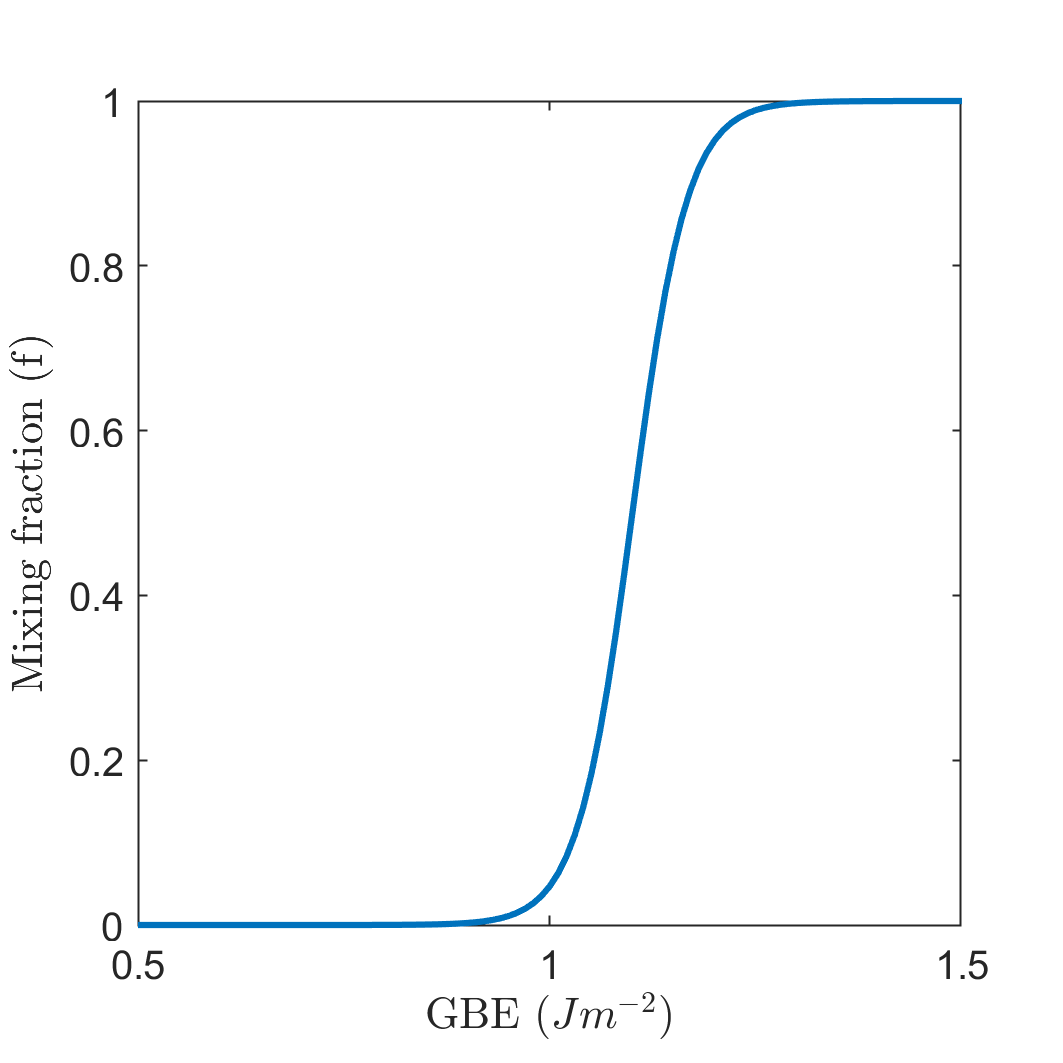
\includegraphics{figures/gprmix-sigmoid.png}
    \caption{Sigmoid mixing function used in the \gls{gpr} mixing model with $m=30$ and $b=\sigthr{}$ (\cref{eq:sigmoid}).}
    \label{fig:gprmix-sigmoid}
\end{figure}

Uncertainty of the \gls{gpr} mixing model is similarly obtained by taking a weighted average of the uncertainties of each model according to:

\begin{equation}
    \sigma_{mix} = f \sigma_1+(f-1) \sigma_2
    \label{eq:gprmix-sigma}
\end{equation}
where $\sigma_1$ and $\sigma_2$ are the corresponding uncertainties of $\epsilon_1$ and $\epsilon_2$, respectively, and f is given by \cref{eq:sigmoid}.

\begin{figure}
    \centering
    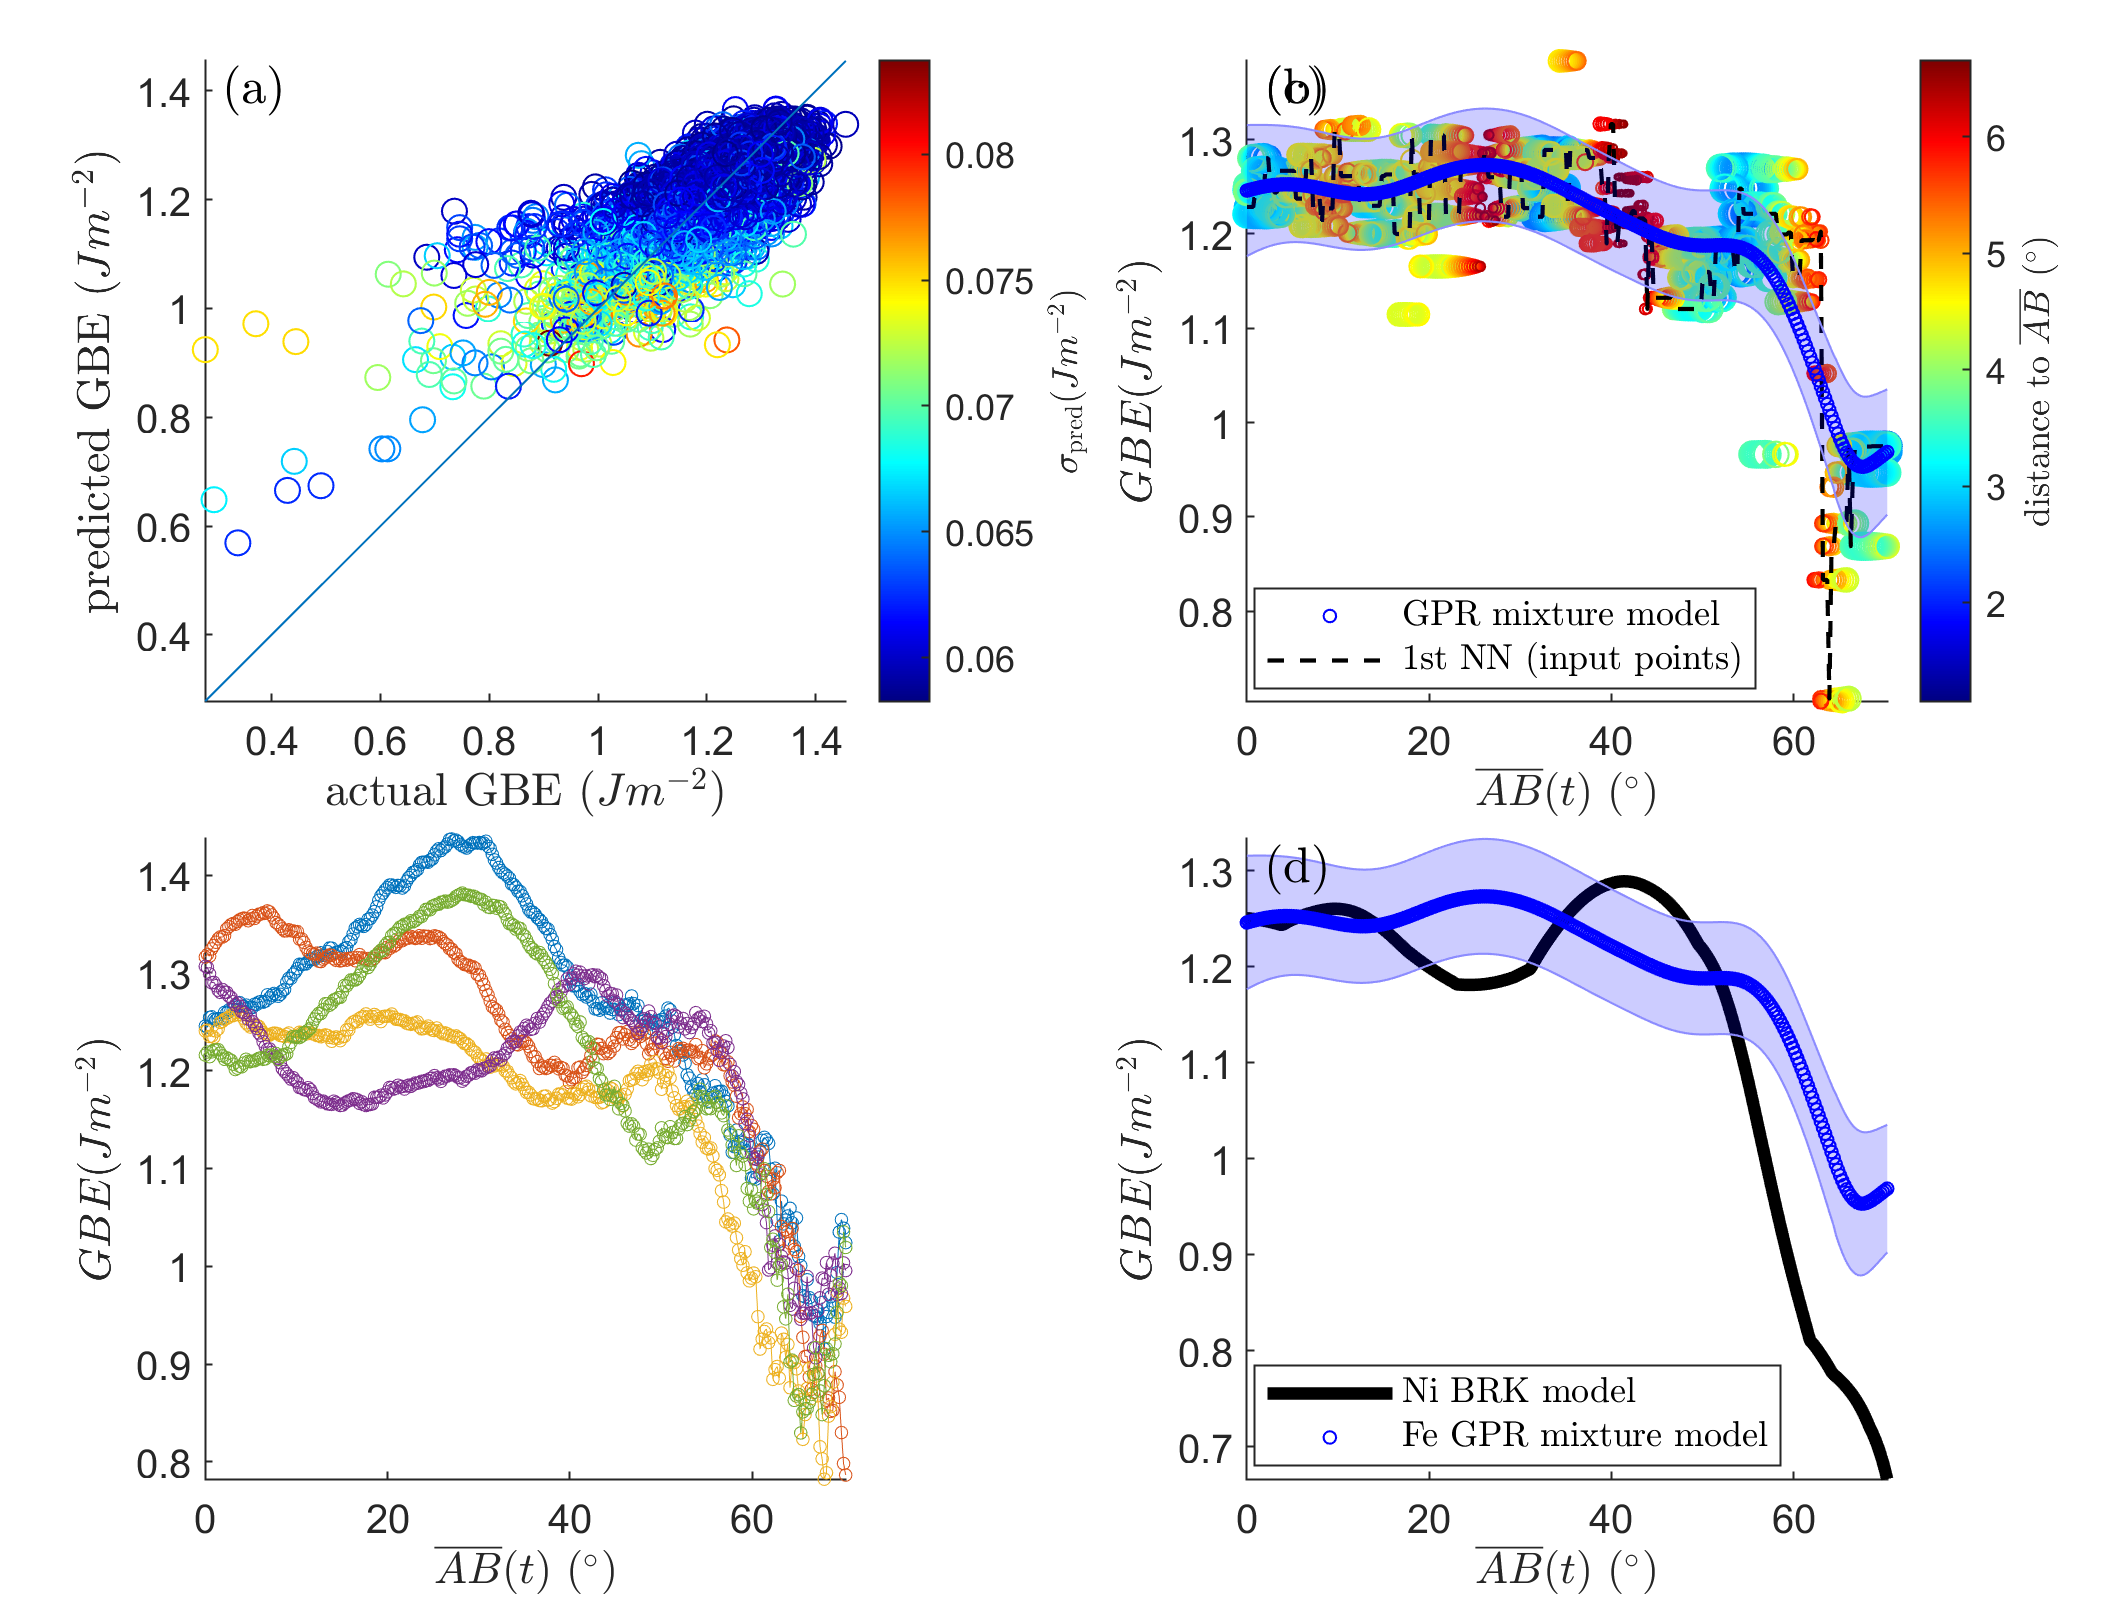
\includegraphics{figures/kim-interp-posterior.png}
    \caption{Interpolation results for a large Fe simulation database \cite{kimPhasefieldModeling3D2014} using \num{46883} \inpt{} \glspl{gb} and \num{11721} \outpt{} \glspl{gb} in an 80\%/20\% split and a \gls{gpr} mixture model to better approximate low \glspl{gbe}. (a) Parity plot colored by uncertainty standard deviation. (b) Prediction (black) and uncertainty standard deviation (grey band) of \gls{gpr} mixture model as a function of distance along a 1D arc ($\overline{AB}$) between two \glspl{vfzo} ($A$ and $B$). The first \inpt{} \gls{nn} is shown as a black, dashed line. The \inpt{} point \glspl{knn} ($k\in[1,2,3,4,5,6]$) relative to $\overline{AB}$ are colored and sized according to the distance to $\overline{AB}$ (\inpt{} points far from the line are small, dark red circles and \inpt{} points close to the line are large, dark blue circles). In other words, this shows the data in a small region of influence around $\overline{AB}$ that contributed to the model predictions where close data is emphasized (larger) than far-away data (smaller). (c)
    Five models sampled from the posterior distribution of the \gls{gpr} mixture model. (d) Fe \gls{gpr} mixture model results and uncertainty standard deviation (grey band) overlaid with the Ni \gls{brk} model along the arc $\overline{AB}$. Coordinates for $A$ and $B$ are given in \cref{tab:tunnel-AB2} of the main paper and 300 equally spaced points are plotted for (b), (c), and (d).}
    \label{fig:kim-interp-posterior}
\end{figure}

\subsection{Input Data Quality}
\label{sec:supp:kim-interp:quality}
By comparing \glspl{gbe} values of (unintentionally) repeated \glspl{gb} in the Fe simulation dataset \cite{kimPhasefieldModeling3D2014}, we can estimate the intrinsic error of the \inpt{} data. First, we see that by binning into degenerate sets, most sets have a degeneracy of fewer than 5 \cref{fig:kim-interp-degeneracy-sets}. We split the repeated data into sets with a degeneracy of fewer than 5 and greater than or equal to 5 and plot the errors (relative to the respective set mean) in both histogram form (\cref{fig:kim-interp-degeneracy-results}a and \cref{fig:kim-interp-degeneracy-results}c, respectively) and as hexagonally-binned parity plots (\cref{fig:kim-interp-degeneracy-results}b and \cref{fig:kim-interp-degeneracy-results}d, respectively). While heavily repeated \glspl{gb} tend to give similar results, occasionally repeated \glspl{gb} often have larger \gls{gbe} variability. This could have physical meaning: Certain types of (e.g. high-symmetry) \glspl{gb} tend to have less variation (i.e. fewer and/or more tightly distributed metastable states). However, it could also be an artifact of the simulation setup that produced this data (e.g. deterministic simulation output for certain types of \glspl{gb}).

\begin{figure}
    \centering
    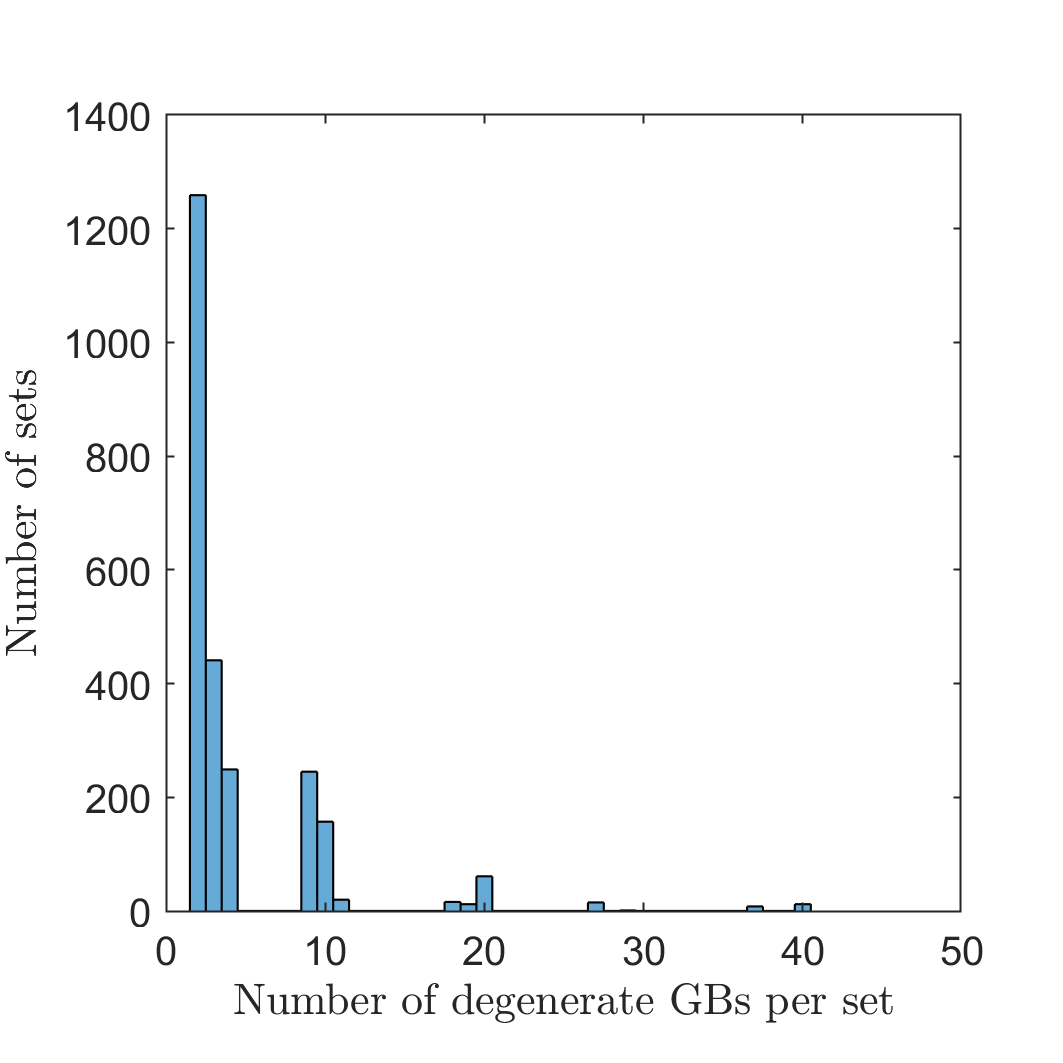
\includegraphics{kim-interp-degeneracy-sets.png}
    \caption{Histogram of number of sets vs. number of degenerate \glspl{gb} per set for the Fe simulation dataset \cite{kimPhasefieldModeling3D2014}. Most sets have a degeneracy of fewer than 5.}
    \label{fig:kim-interp-degeneracy-sets}
\end{figure}

\begin{figure}
    \centering
    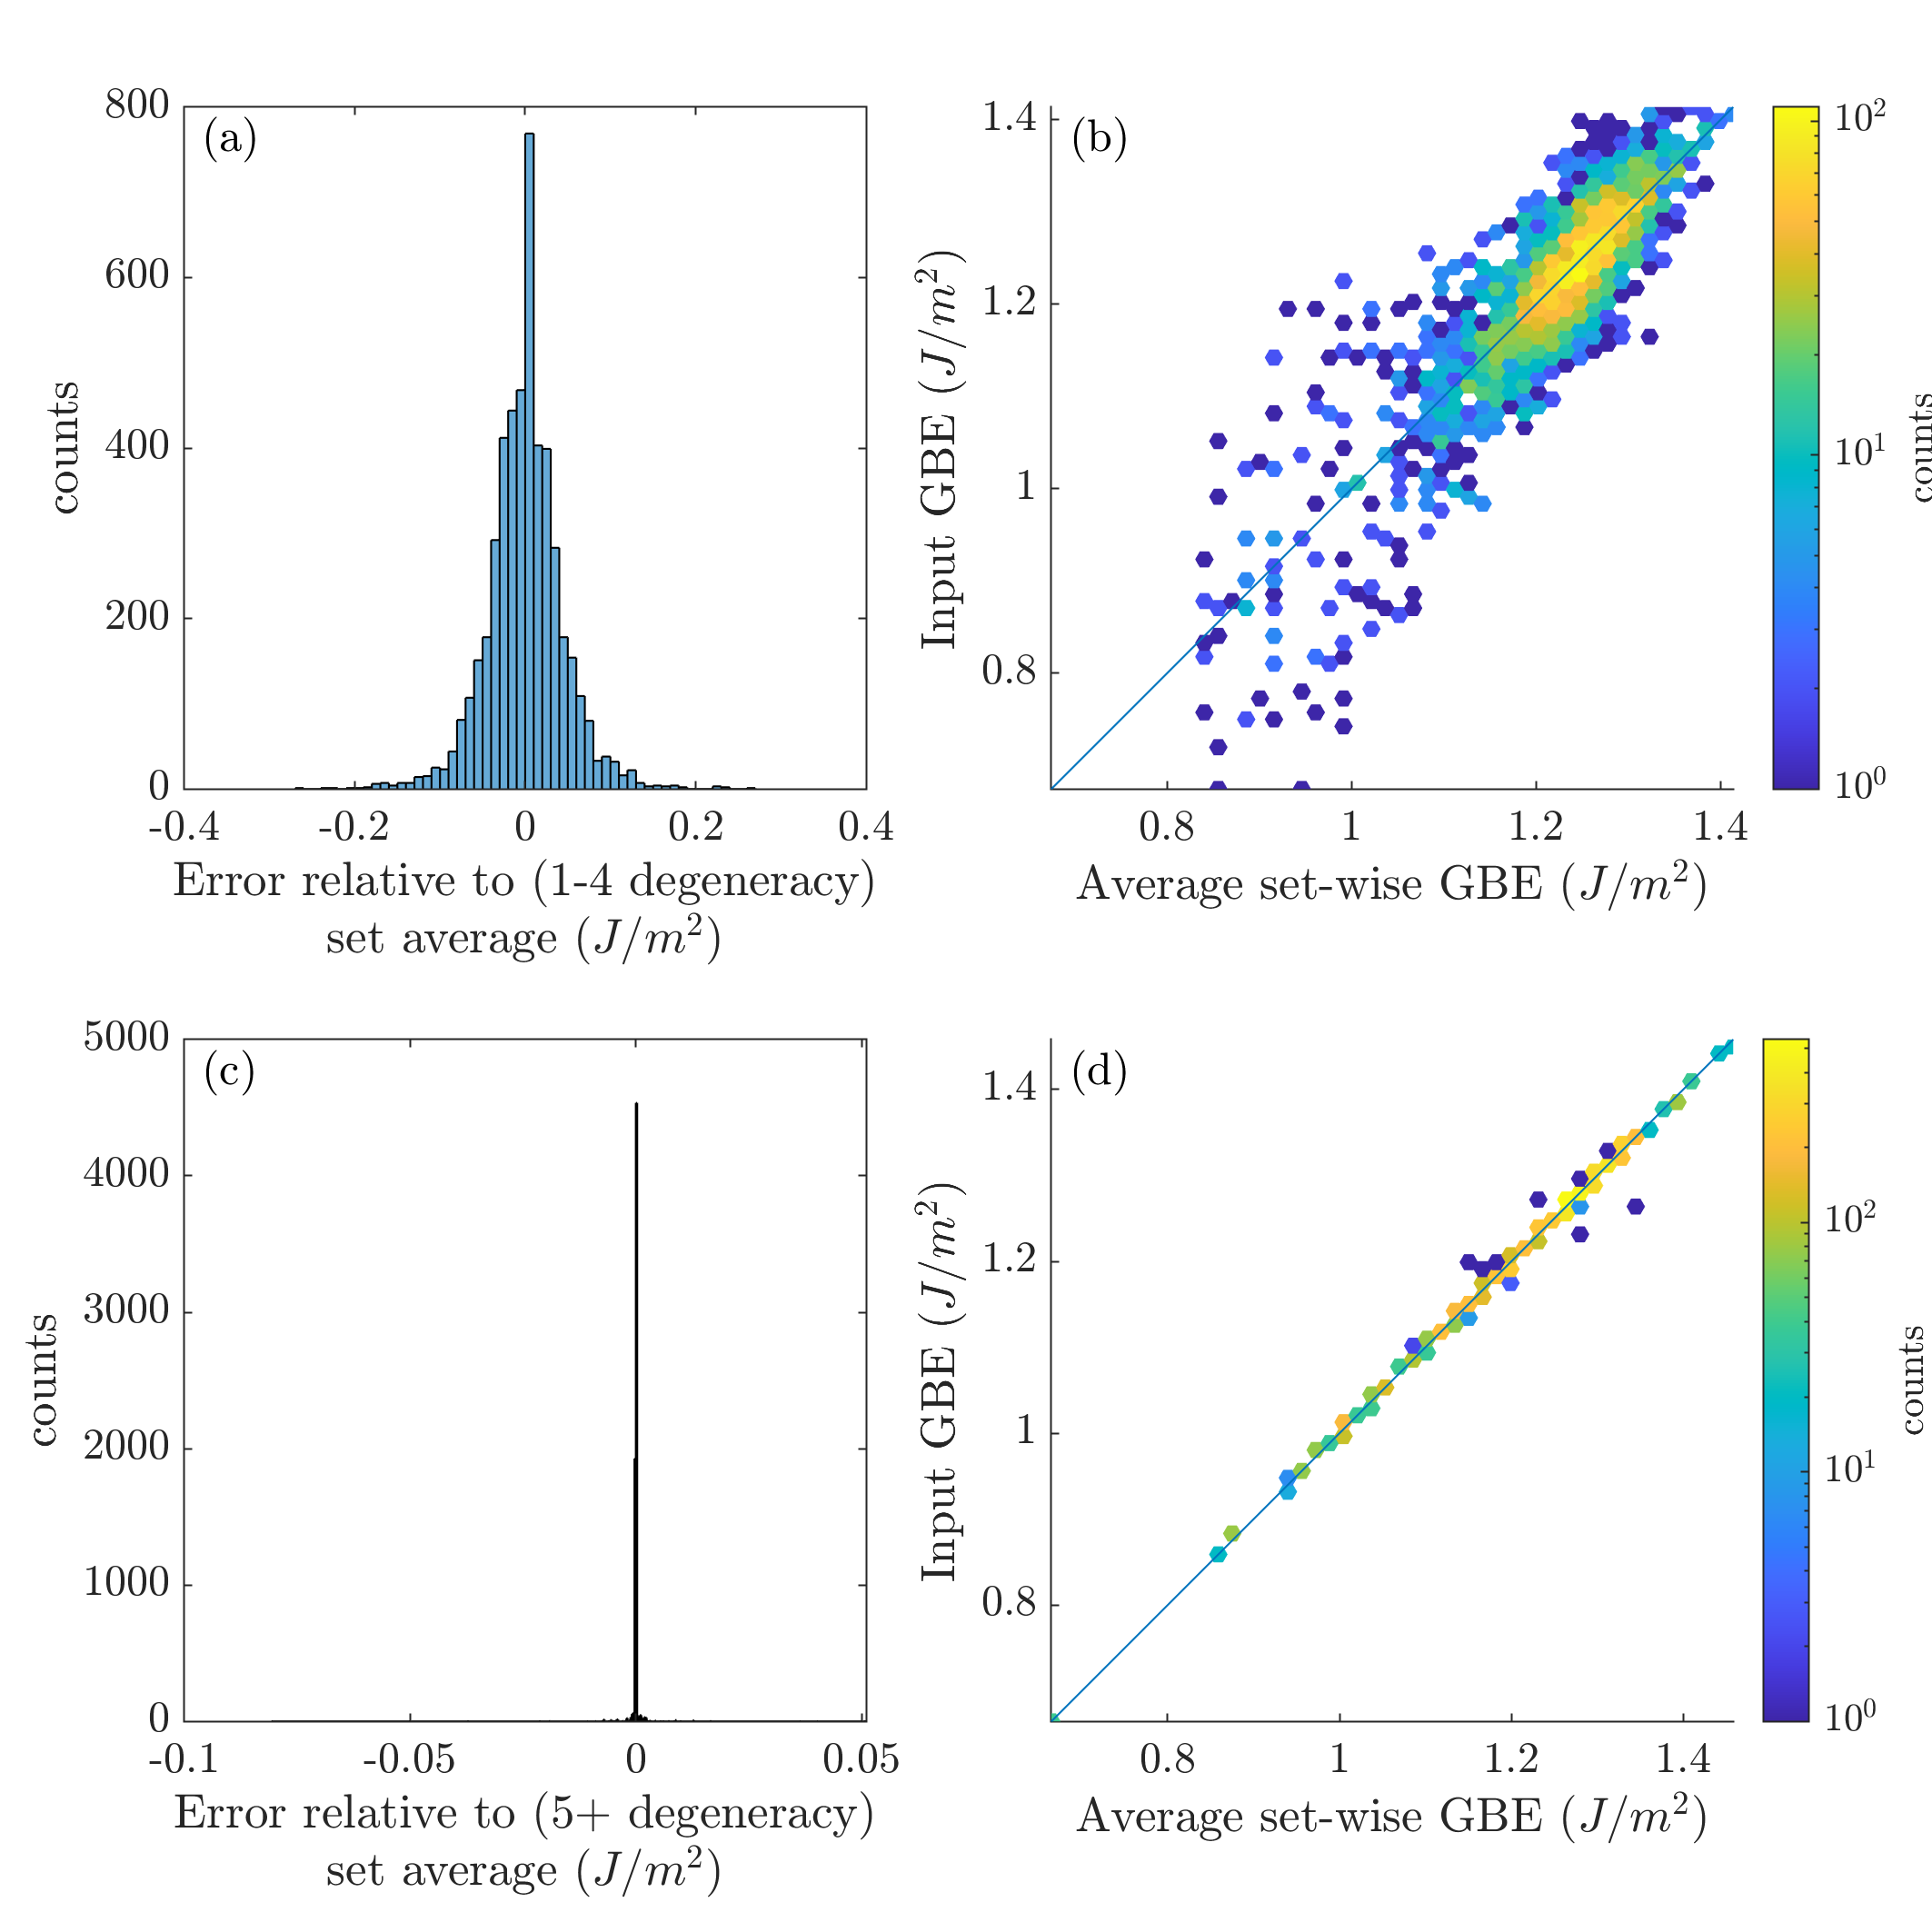
\includegraphics{kim-interp-degeneracy-results.png}
    \caption{Degenerate \glspl{gb} sets are split into those with a degeneracy of fewer than 5 and greater than or equal to 5 and plotted as error histograms ( (a) and (c), respectively) and hexagonally-binned parity plots ( (b) and (d), respectively.). Large degenerate sets tend to have very low error, whereas small degenerate sets tend to have higher error. In other words, \glspl{gb} that are more likely to be repeated many times based on the sampling scheme in \cite{kimPhasefieldModeling3D2014} tend to give similar results, whereas \glspl{gb} that are less likely to be repeated often have larger variability in the simulation output. We do not know if this has physical meaning or is an artifact of the simulation setup.}
    \label{fig:kim-interp-degeneracy-results}
\end{figure}

%The true, underlying \gls{brk} function is also shown (black line) and a shaded error band of uncertainty standard deviation. \glspl{knn} ($1<=k<=6$) \inpt{} points closest to $\overline{AB}$ are plotted and colored by distance to $\overline{AB}$.

% \newpage
% \printglossaries
%need to manually clear cached files & logs in overleaf to get updated abbreviations to appear

\newpage
\clearpage
\bibliographystyle{elsarticle-num-names}
\bibliography{5dof-gb-energy.bib}

\end{document}